\section{Evaluation}
\subsection{Generated-signal reliability}
The signal suite pairs twelve conditions within each of \BenchTrials{} explicit
scenario seeds: uniform force-noise bounds of 0, 100, 300 and 600 mN crossed with
uniform contact-duration jitter bounds of 0, 10 and 30 ms. It performs
\ChannelObservations{} generated trace trials. Success means that an honest
controller's \texttt{respond} routine accepts the trace, recomputes the pattern
and emits a signed response. Failure reasons and processing costs are retained.
No physical sensor, person or actuator participates.

\begin{figure*}[t]
\centering
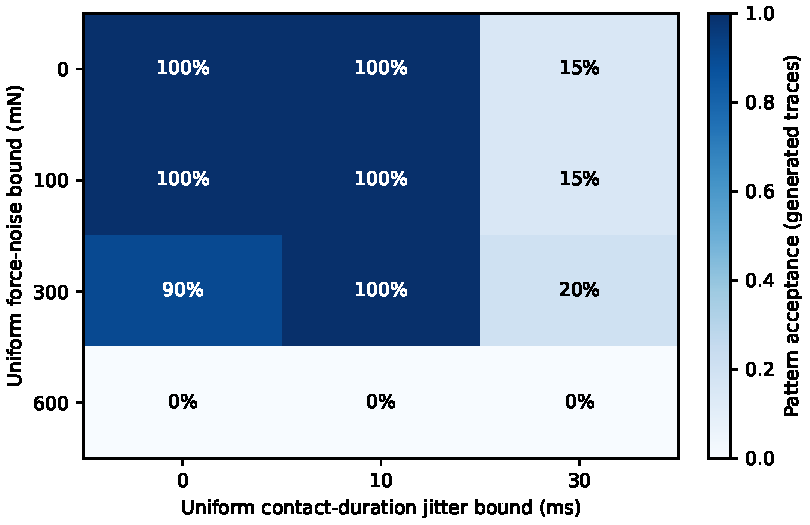
\includegraphics[width=0.75\textwidth]{artifacts/channel.pdf}
\caption{Pattern acceptance on generated force/time traces. Each cell contains
20 scenario seeds; conditions share seeds. The data describe fixture-profile
sensitivity, not a human-authentication rate or sensor accuracy.}
\label{fig:signal}
\end{figure*}

The zero-noise, zero-jitter condition accepted
\CleanSuccesses{}/\BenchTrials{} traces. Large timing variation reduced acceptance;
600 mN noise produced no accepted traces in the recorded conditions. Not every
intermediate condition is monotonic because noise changes crossing times in a
thresholded signal. The fixed finite scenario family does not support a general
noise-tolerance threshold. Rejected-trace processing is often faster than valid
signing, so pooled timing must not be interpreted as a throughput advantage.
Processing time excludes the simulated multi-second interaction duration.

\subsection{Short-pattern collision experiment}
We preserve one generated old trace and test it against \CollisionTrials{}
different challenge contexts. Its segment pattern matched
\PatternCollisions{} contexts. This is compatible with a small 256-code space,
not a cryptographic break. An old signed envelope still contains its original
nonce/session and fails full binding in a new stored interaction. Conversely, a
controller that signs old raw samples for a colliding new pattern can pass the
software checks. Capture freshness is an acquisition assumption, not a property
established by the eight tactile bits. The benchmark records this negative
result explicitly.
\subsection{Policy controls and schedules}
The serial suite repeats every named case \BenchTrials{} times with fresh keys,
challenges and temporary SQLite state. It includes changed principals, actions,
resources, purposes and arguments; altered signatures; unconfigured keys; session
and nonce transplantation; wrong audience; expired challenges and grants; grant
and issuer revocation; unregistered permission; wrong grant scope/modality;
consumed replay; malformed observation profiles; unsupported guarantees and
unaccepted assumptions. Modality-specific cases extend this common taxonomy.

An intentionally weak signature-only ablation ignores scope, freshness and
permission. It isolates why authentication alone is insufficient; its failures
are not evidence against correctly configured existing authorization. An equally
expressive sequential typed-policy control separately checks the same expected
challenge, action, supported guarantees and permission state. It shares
cryptographic and modality validators with the gateway and is not an independent
audit, full IFC implementation or reimplementation of published agent defenses.

The concurrency suite runs \BenchTrials{} trials of eight duplicate attempts
released together; each must produce exactly one receipt. Another
\BenchTrials{} trials hold the write boundary, revoke the grant and then release a
worker's commit. Every such prior-revocation schedule must produce zero receipts.
This is a deliberately selected serialized order, not an exhaustive scheduler
exploration. Tests also check rollback, expiry at the boundary and replay after
restart.

\subsection{Interpretation}
Across \SecurityObservations{} serial case observations
(\SecurityCases{} cases per trial), the gateway produced
\UnauthorizedEffects{} unauthorized new local receipts and
\TypedDisagreements{} disagreements with the typed control. The weak
signature-only check accepted \SignatureFalseAccepts{} observations that violated
the specified policy. Mixed accepted/denied gate processing had median
\GateMedian{} ms and nearest-rank p95 \GatePninetyfive{} ms. These one-host
measurements include SQLite work for accepted requests, but are not a matched
latency comparison with the control or an end-to-end physical delay.

Two limitation cases deliberately accept valid structured responses: transparent
live forwarding when no proximity guarantee is required, and a configured
attester producing a plausible report when sensor truth is not required. These
are modeled traces, not physical relay or compromised-device experiments. Requiring
proximity or consent is separately denied. Denial is not a result demonstrating
those properties. Channel trials and policy cases are distinct suites; the
runnable demos combine channel parsing, signature appraisal and effect insertion.

\subsection{Validity and missing measurements}
Signal seeds are deterministic, key material and security challenges are fresh,
and all processing measurements come from one host. The force model, thresholds
and attack schedules were selected by the implementation authors. Per-condition
Wilson intervals are descriptive; paired conditions are not independent trials
that can be pooled into a deployment security rate. We have not measured real
force calibration, skin/material variation, user behavior, motor control,
controller compromise, haptic relay, classifier discrimination or secure hardware.
Future studies require those measurements and independent review before claiming
physical reliability or human authorization.

